\section{System Overview}
\subsection{Extensions to the core system classes}
%
\begin{figure}[bt]
  \begin{center}
    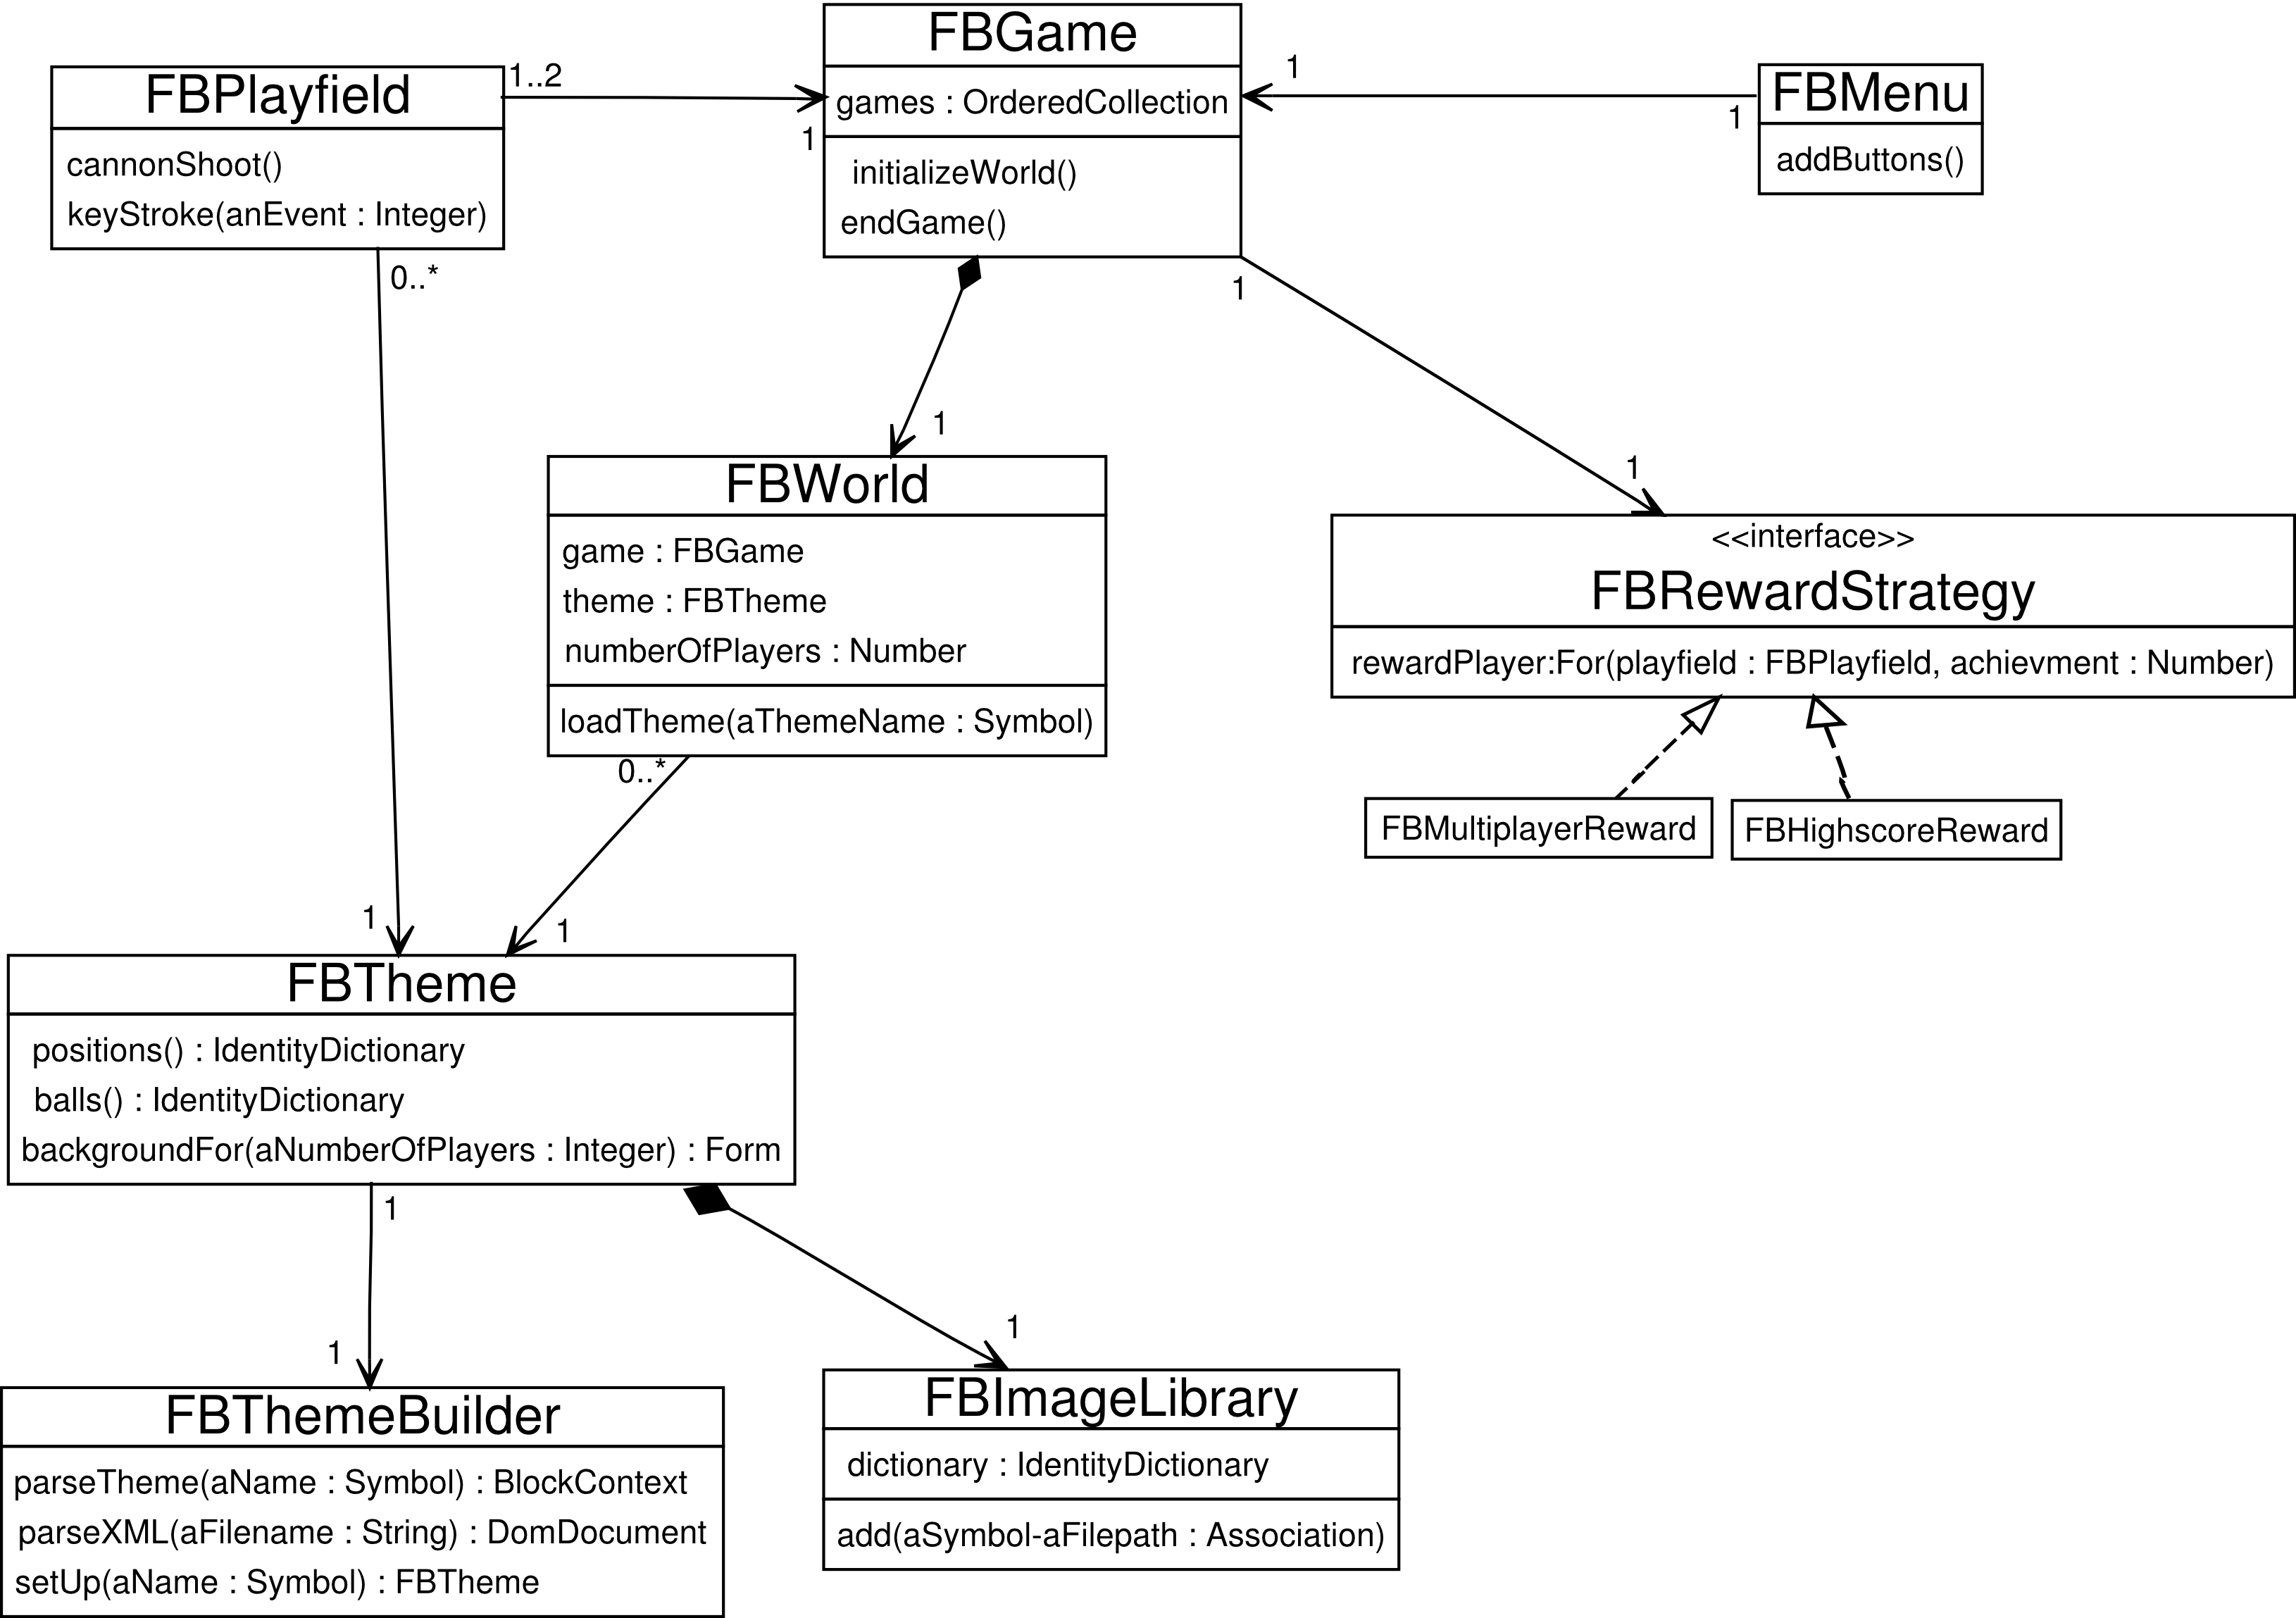
\includegraphics[width=\linewidth]{images/systemcore.png}
  \end{center}
  \caption{The extended core system}
  \label{fig:systemcore}
\end{figure}
%
\subsubsection{Rewarding the Players} ~\\
FBRewardStrategies are supporting objects which add rewarding behaviour 
to the game logic
~(Fig.\ref{fig:systemplay}). Its specializations 
implement different strategies to
reward the players for good gaming. Good gaming is measured by the 
number of balls falling, if more are falling at the same time, more 
reward points are gained.
The reward strategies have to implement a method
rewardPlayer:for:~(Listing \ref{lst:reward}).\\
In single player mode, a FBHighscoreReward
adds a simple highscore to the screen (responsible for adding the 
score visual is also the strategy itself) and for any number of 
reward points reported by the FBPlayfield, score points are accumulated.
%
\begin{lstlisting}[float,label=lst:reward,caption=The Highscore Calculation Method]
FBHighscoreReward>>rewardPlayer: aPlayer for: anAchievmentScalar
    "I reward a single player with an exponentially 
rising rate of points" 

    self score:
         self score + (anAchievmentScalar raisedTo: 2)
\end{lstlisting}
%
In multiplayer mode, the strategy only rewards, if the player eliminates 
more than three balls from the field with a single shot. If that happens, 
a number of balls half as great is distributed among the other players,
and shot randomly in any direction. This happens via a call to 
the playfields which have to shoot random balls, since FBRewardStretegies
hold a collection referring to all playfields.
%
\subsubsection{FBTheme and FBImageLibrary}~\\ 
To avoid expensive reading from hard disk as mentioned in our design solutions~(\ref{sec:theme})
we implemented the FBTheme class as a flyweight, holding references to previously 
created instances of a particular theme. If a requested theme type is not yet 
held in the list of instances~\ref{lst:theme}, the class calls a builder class, 
FBThemeBuilder~\ref{fig:systemcore}, to parse the requested theme's XML file, 
load the images and then return a fresh instance of the theme. Additionally, 
each theme contains an FBImageLibrary. The image library is just a simple 
wrapper around an IdentityDictionary to ease filling it with Forms. 
FBTheme and FBImageLibrary also support scaling to adjust to any screen 
size (without accounting for necessary interpolation).
The FBImageLibrary is filled prior to starting the actual game, so 
that all external resources are cached. A lazily initialized image 
library would have resulted in slow disk I/O during
run-time.
%
\begin{lstlisting}[language=Smalltalk, label=lst:theme, caption= FBTheme "return:" method, float]
FBTheme class>>return: aSymbol
    "Return the instance of the requested type if we have it. If not replace any old instance with the type requested."
    instances ifNil: [instances := IdentityDictionary new].
    ^ instances 
        at: aSymbol 
        ifAbsent: [
            | instance |
            instance := self builder setUp: aSymbol.
            (instances add: aSymbol -> instance) value].
\end{lstlisting}
%
\subsection{FBPlayfield and associated classes}
%
\begin{figure}[bt]
  \begin{center}
    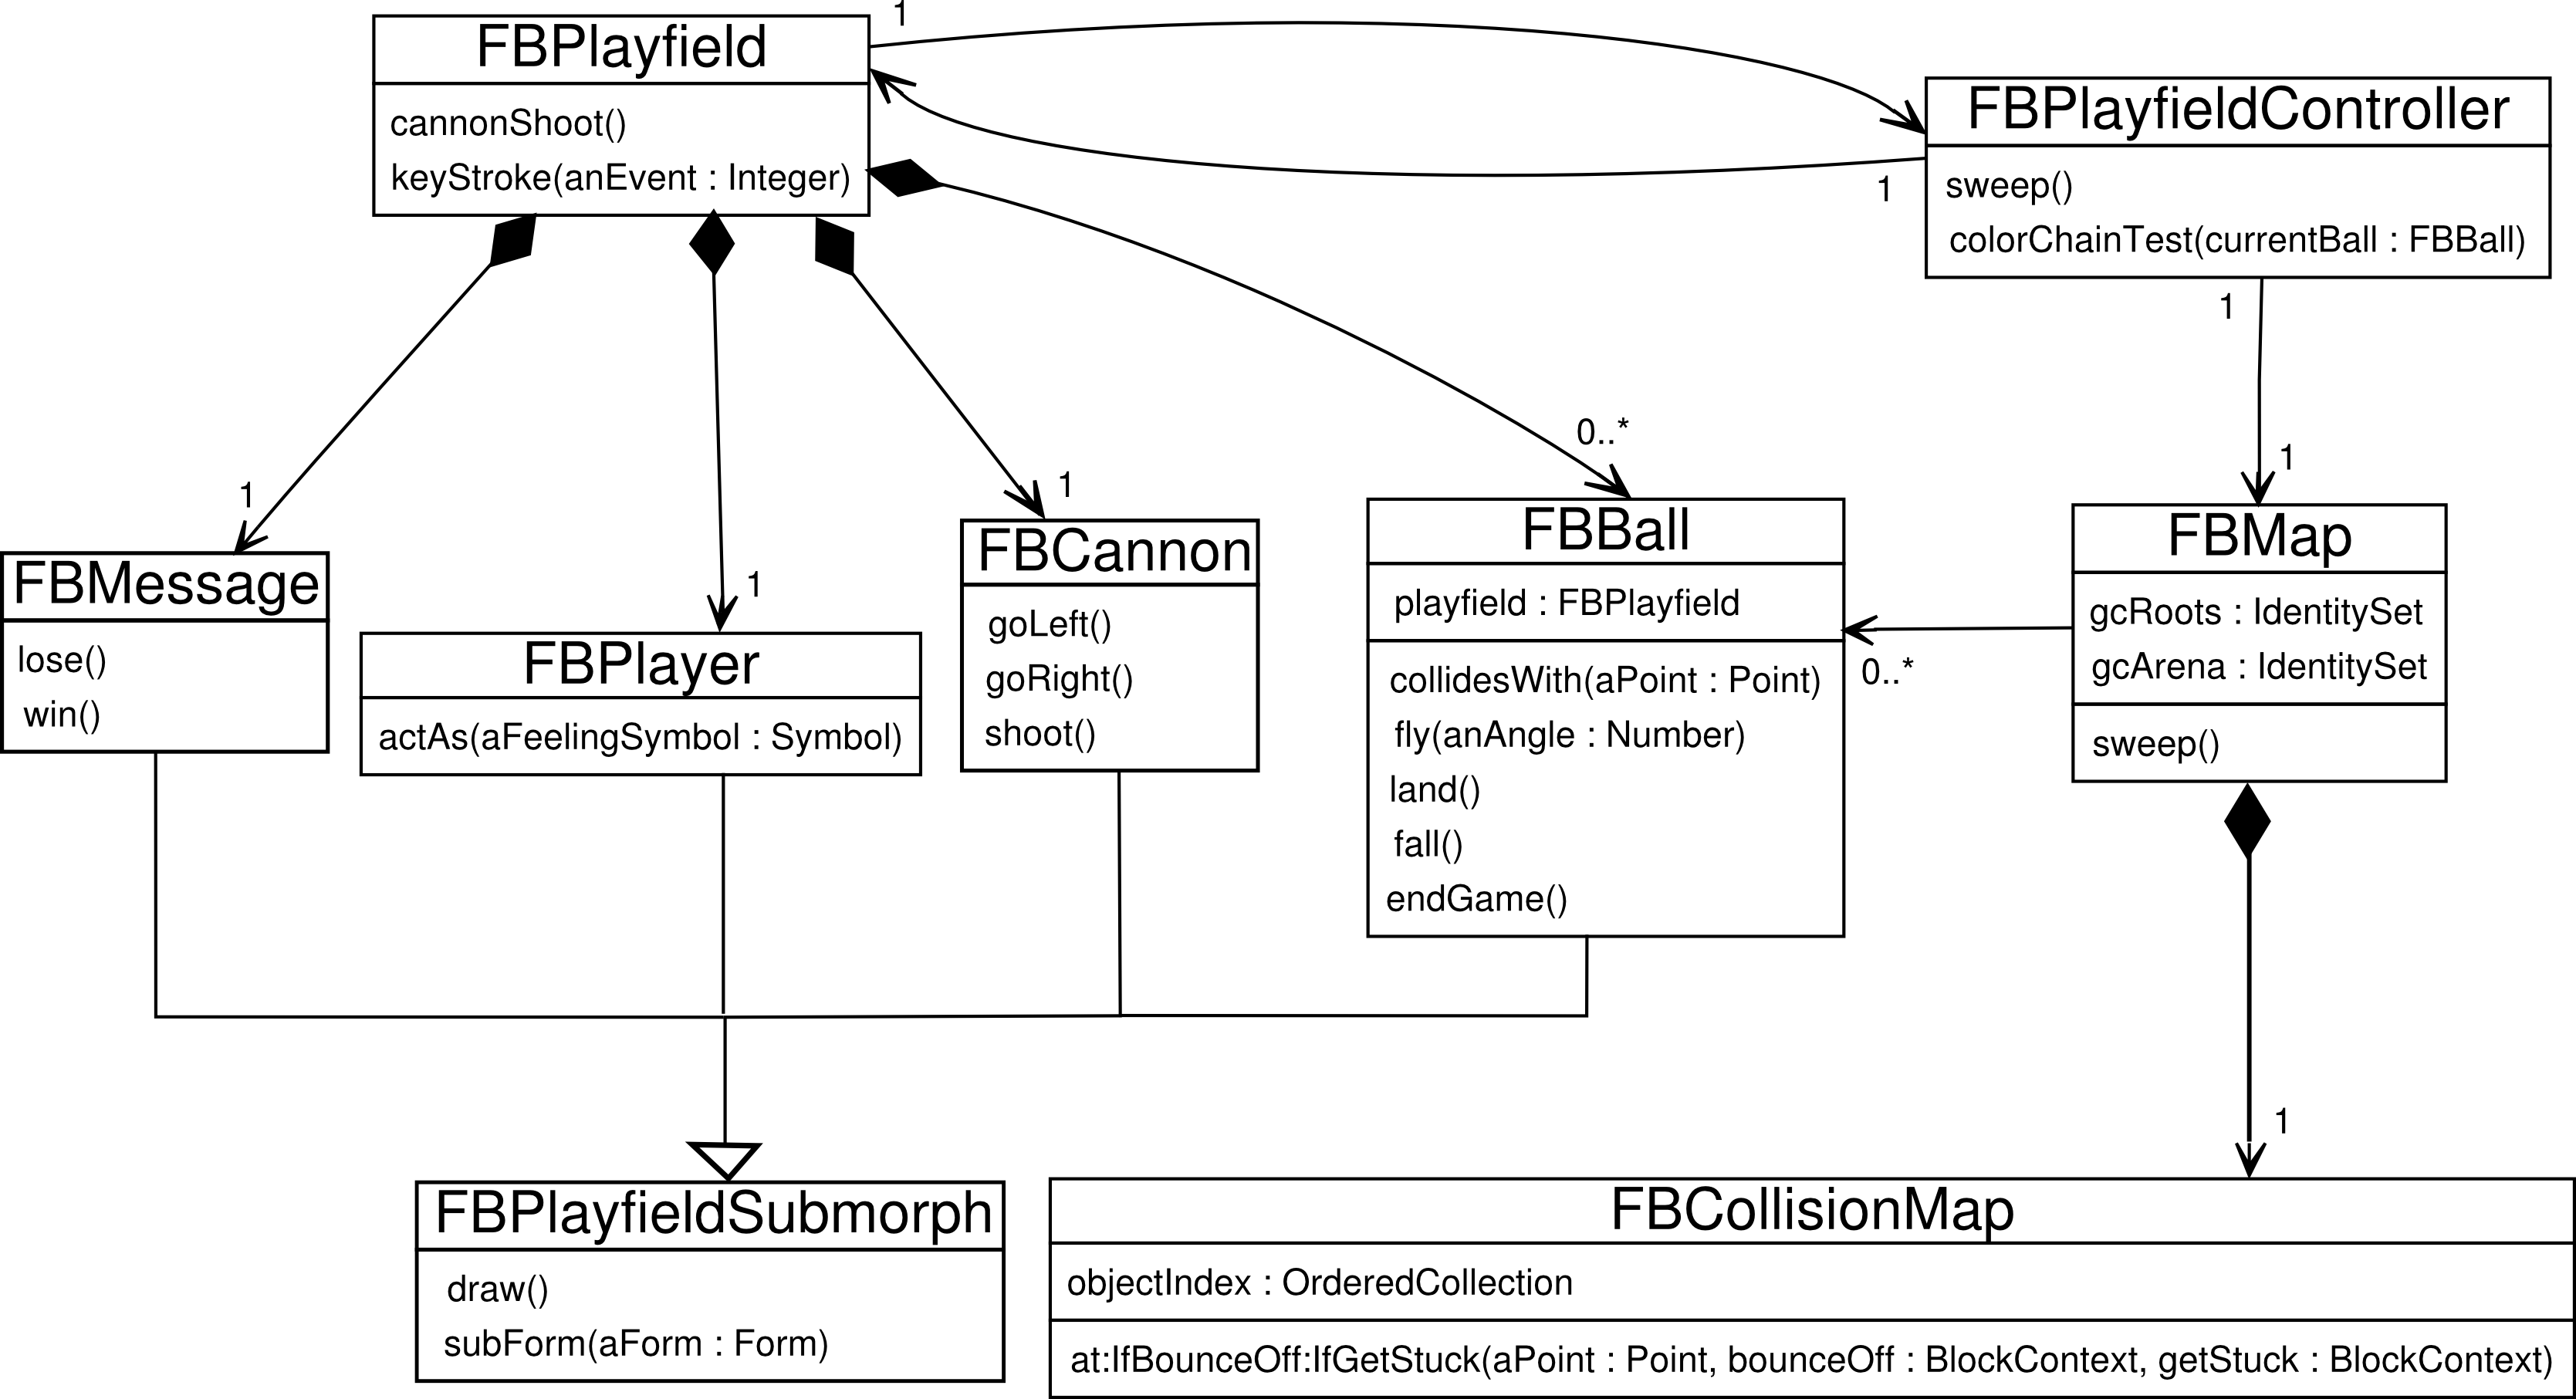
\includegraphics[width=\linewidth]{images/systemplay.png}
  \end{center}
  \caption{The classes connected to each playfield}
  \label{fig:systemplay}
\end{figure}
%
\subsubsection{Playfield Morphs}~\\
As aforementioned, FBPlayfield is responsible for creating its own 
contents~(\ref{fig:systemplay}). Such content displays a cannon, a 
player avatar, messages for the user and numerous coloured balls. 
Each of these serves only a single, limited purpose, with FBPlayer 
and FBMessage merely wrapping different types of graphical interaction.
The cannon is the entity that reacts to the user's input, panning 
left and right and sending balls off into the field. However, it 
is controlled entirely by the playfield and does not act itself. 
The FBBall is an exception to this simplicity. 
Because of that, we decided to separate all logic concerning falling
FBBalls from the rest of the playfield and provide an additional
abstraction layer, FBPlayfieldController.


\begin{description}
  \item[First]
    	it has to look 
	differently, showing different colors in our themes. 
  \item[Secondly]
    	a Ball has different stages in its lifetime, being 
	loaded into the cannon, then flying, hanging from the 
	ceiling (or, indeed, from other balls) and finally falling 
	and vanishing.
  \item[Finally]
    	a Ball needs to collide with the playfield boundaries and 
	other balls in the field.
\end{description}
Thus its implementation is a bit larger, as it implements the FBCollider 
interface, utilizes different ``states'' to act on in its step method and 
and also draws itself from a collection of images.
%
\subsection{FBMap}
\subsubsection{Collision Detection}
As mentioned in section
\ref{sec:collision}, 
\label{sec:collisionmap}
collision detection is handled by one collision map per playfield. This collision
map is an instance of FBCollision. A collision is detected a posteriori, meaning
that the ball first moves to the next position and  than checks whether it collides
with some other object. However, this is not strictly necessary and not reflected in
the implementation of the collision map. Any object may ask the collision map whether
a collision is happening at a given point on the map and may react accordingly. There
are two kinds of collision: One where a ball usually should get stuck and one where it
should bounce of. As can be seen in Listing \ref{lst:ifBounceOff}, the API call wraps
around doYouGetStuckAt: and doYouBounceOff: - checking in that order, since if a ``stuck
collision'' should occur, it has a higher priority than a ``bounce of collision''.
% 
\begin{lstlisting}[caption=API method for detecting collision,label=lst:ifBounceOff]
FBMap>>at:aPoint ifBounceOff:bounceOffBlock ifGetStuck:getStuckBlock
	
	(self doYouGetStuckAt: aPoint)
		ifTrue: [getStuckBlock value]
		ifFalse: [ (self doYouBounceOff: aPoint)
			ifTrue: bounceOffBlock ]
\end{lstlisting}
%
Up to this point the API is independent from how an collision is actually detected.
The playfield is divided grid, each cell being the size of a ball. Those cells are represented
in the objectIndex collection. Each ball that lands somewhere registers on all cells where
another ball could possibly collide with it, which are all the cells that are direct neighbours
of the cell in which the ball landed. Note that the cell a ball ``is in'' is the cell the ball's
center is in. Now doYouGetStuckAt: aPoint returns true if one of the balls registered on the
cell aPoint is in, would collide with a ball with a center at aPoint (or if the ball would be
close enough to the upper border). So instead of comparing with all balls on the playfield, which
would be the most trivial implementations, we only compare the current position to the position
of the balls near by. Since a cell is the size of a ball, there can only be up to 8 balls surrounding
a cell, independent of playfield size or total number of balls. Therefor, collision detection is in
$O(1)$ complexity, compared to $O(n)$ of the trivial implementation.

As mentioned in \ref{sec:collision}, an alternative implementation could have been pre- computing the route
with vectors. However, this has at least two downsides. First, it does not cope with changes happening
while the ball is flying. But this is not likely to happen. The other downside is, that it does need more
computation than our solution. Not only would we need some concept of vectors, we would also have to check
with every ball on the playfield or use some grid algorithm like the one we are using for our implementation.
Thus we would have the computation we already have plus the vector algorithms. The advantage would be to avoid
collision detection computation while the ball is flying. However, profiling did show that this would probably
not lead to an performance boost. Moreover, our current implementation does not check for every pixel lying
on the way, but only for those where it will ``jump'' to on every step, so we have less comparisons than compared
to the vector approach. Not checking for every pixel forces us to readjust the position as soon as the ball got stuck.
%
\subsubsection{Ball Falling Conditions}
As discussed in section \ref{sec:garbage}, we modeled the process to decide whether balls can fall down on garbage collection. Our first design was inspired by reference-counting and planned for every ball to keep track of all objects it holds on to and all objects that hold on to it. When an object falls down, it informs the objects that hold on to it, via the Squeak built-in event mechanism~\cite{website:squeakwikiObserver}, that they lost a holder. When an object has lost its last holder, it should itself fall down and inform all objects that hold on to it that it is gone.
This approach had several drawbacks. First, the logic for this falling down was distributed over the FBCollisionMap, FBBall and FBCollider\footnote{This class had only been needed with the reference counting approach and was discarded for the final version.} classes.
Second, every Ball observed the Balls next to it. When a Ball was removed from the structure, the observing Balls removed it from their lists of holders. In the event that a Ball had no holders, it fell down, thereby invoking events on its observing neighbours.
This resulted in a control flow that was hard to understand, as the information of the removal of a Ball was propagated to the other Balls implicitly through events and not explicitly through messages.

Third, reference-counting garbage collectors have a well-known problem with cyclic references.

In order to separate the concern of letting balls fall down the from the rest of the game logic, the FBMap keeps track of the balls and the relationships between them.

Like a mark-and-sweep garbage collector, the sweepBalls method traverses the balls in the Playfield and marks every ball it can reach, beginning with the balls that stick to the top of the playfield. The Balls are traversed depth-first. All unmarked balls cannot be reached from balls that hang. They are removed from the map.

%
\begin{lstlisting}[language=Smalltalk, label=lst:sweep, caption=Mark-and-Sweep Ball Collector, float]
FBMap>>sweepBalls
	"Grep chains for all roots and remove the rest"
	
	| markedColliders removableColliders |
	markedColliders := gcRoots copy.
	self gcRoots do: [:each | 
		markedColliders addAll: (self 
			chainFor: each 
			except: markedColliders)].
	removableColliders := (self
			ejectAll: markedColliders
			from: self gcArena).
	removableColliders do: [:each | self remove: each].
	^ removableColliders
\end{lstlisting}
%
